\documentclass[11pt,a4paper]{article}

% Image mode: pdf.
% Image paths stay relative. In PDF mode, place same-basename PDF conversions
% of the chapter SVG files in the assets/ directory beside this source.

\usepackage{iftex}
\ifPDFTeX
  \PackageError{handout}{This template requires XeTeX or Tectonic}{Compile with xelatex or tectonic.}
\fi

\usepackage[a4paper,top=18mm,bottom=20mm,left=20mm,right=20mm,headsep=6mm]{geometry}
\usepackage{fontspec}
\usepackage{xeCJK}
\usepackage{amsmath}
\usepackage{unicode-math}

% Font settings are intentionally visible in the generated .tex file.
% These defaults target the macOS machine used for the released PDF.
% Change the family names when compiling on another system.
\setmainfont{Songti TC}
\setsansfont{Heiti TC}
\setmonofont{Menlo}
\setCJKmainfont{Songti TC}
\setCJKsansfont{Heiti TC}
\setCJKmonofont{Heiti TC}
\setmathfont{STIX Two Math}
\XeTeXlinebreaklocale "zh"
\XeTeXlinebreakskip=0pt plus 1pt

\usepackage{xcolor}
\definecolor{HandoutBlue}{HTML}{215A91}
\definecolor{HandoutBlueLight}{HTML}{EEF5FC}
\definecolor{HandoutGreen}{HTML}{39715A}
\definecolor{HandoutGreenLight}{HTML}{EFF8F3}
\definecolor{HandoutGold}{HTML}{8A641C}
\definecolor{HandoutGoldLight}{HTML}{FFF8E8}
\definecolor{HandoutInk}{HTML}{253142}
\definecolor{HandoutMuted}{HTML}{667085}

\usepackage{graphicx}
\makeatletter
% Pandoc 3 emits an accessibility `alt` key for raster/PDF images. Older
% graphicx releases do not know that key, so accept it without changing layout.
\@ifundefined{KV@Gin@alt}{\define@key{Gin}{alt}{}}{}
\newsavebox\pandoc@box
\newcommand*\pandocbounded[1]{%
  \sbox\pandoc@box{#1}%
  \Gscale@div\@tempa{\textheight}{\dimexpr\ht\pandoc@box+\dp\pandoc@box\relax}%
  \Gscale@div\@tempb{\linewidth}{\wd\pandoc@box}%
  \ifdim\@tempb\p@<\@tempa\p@\let\@tempa\@tempb\fi
  \ifdim\@tempa\p@<\p@\scalebox{\@tempa}{\usebox\pandoc@box}%
  \else\usebox{\pandoc@box}%
  \fi
}
\makeatother
\usepackage{float}
\floatplacement{figure}{H}
% Pandoc uses LTcaptype=none for uncaptioned longtables. The caption package
% expects that name to exist as a counter even though it is never displayed.
\newcounter{none}
\usepackage{caption}
\captionsetup[figure]{labelformat=empty,labelsep=none,font=small}

\usepackage{booktabs,longtable,array,calc}
\usepackage{etoolbox}
\makeatletter
\patchcmd\longtable{\par}{\if@noskipsec\mbox{}\fi\par}{}{}
\makeatother

\usepackage[most]{tcolorbox}
\tcbuselibrary{breakable,skins}
\newtcolorbox{HandoutLearningMap}{
  enhanced,breakable,colback=HandoutBlueLight,colframe=HandoutBlue,
  boxrule=0.8pt,arc=1.5mm,left=3mm,right=3mm,top=2mm,bottom=2mm,
  before skip=8pt,after skip=10pt
}
\newtcolorbox{HandoutWorkedExample}{
  enhanced,breakable,colback=HandoutGreenLight,colframe=HandoutGreen,
  boxrule=0.65pt,arc=1.5mm,left=3mm,right=3mm,top=2mm,bottom=2mm,
  before skip=8pt,after skip=10pt
}
\newtcolorbox{HandoutSelfCheck}{
  enhanced,breakable,colback=HandoutGoldLight,colframe=HandoutGold,
  boxrule=0.65pt,arc=1.5mm,left=3mm,right=3mm,top=2mm,bottom=2mm,
  before skip=8pt,after skip=10pt
}

\usepackage{titlesec}
\titleformat{\section}{\sffamily\bfseries\Large\color{HandoutBlue}}{}{0pt}{}
\titleformat{\subsection}{\sffamily\bfseries\large\color{HandoutInk}}{}{0pt}{}
\titleformat{\subsubsection}{\sffamily\bfseries\normalsize\color{HandoutInk}}{}{0pt}{}
\titlespacing*{\section}{0pt}{1.4em}{0.55em}
\titlespacing*{\subsection}{0pt}{1.15em}{0.45em}
\titlespacing*{\subsubsection}{0pt}{0.9em}{0.35em}
\setcounter{secnumdepth}{-\maxdimen}

\usepackage{hyperref}
\usepackage{bookmark}
\IfFileExists{xurl.sty}{\usepackage{xurl}}{}
\urlstyle{same}
\hypersetup{
  colorlinks=true,
  linkcolor=HandoutBlue,
  urlcolor=HandoutBlue,
  citecolor=HandoutBlue,
  pdftitle={數A3-3 平面向量},
  pdfsubject={數學},
  pdfcreator={Pandoc with the HighSchooContent LaTeX template}
}

\setlength{\parindent}{0pt}
\setlength{\parskip}{0.55em plus 0.15em minus 0.1em}
\setlength{\emergencystretch}{3em}
\setlength{\LTpre}{0.5em}
\setlength{\LTpost}{0.5em}
\renewcommand{\arraystretch}{1.18}
\providecommand{\tightlist}{%
  \setlength{\itemsep}{0pt}\setlength{\parskip}{0pt}}
\pagestyle{plain}


\begin{document}

\begin{tcolorbox}[
  enhanced,colback=white,colframe=HandoutBlue,boxrule=1.1pt,arc=2mm,
  borderline west={3pt}{0pt}{HandoutBlue},left=5mm,right=4mm,top=4mm,bottom=4mm
]
{\sffamily\small\bfseries\color{HandoutBlue}學生講義}\par
{\sffamily\bfseries\LARGE\color{HandoutInk}數A3-3 平面向量}\par
\vspace{0.35em}{\large 把方向變成可運算的分量，再用內積與行列式讀角度和面積}\par
\vspace{0.45em}{\small\color{HandoutMuted}%
科目：數學
\quad 課程：普通高中數學A 第三冊
\quad 版本：學生版｜核心＋理解
\quad 校訂：2026-08-29
}\par
\vspace{0.25em}{\small\color{HandoutMuted}範圍：現行數學A主線}\par
\end{tcolorbox}


\begin{HandoutLearningMap}

\subsection{本章核心問題}\label{ux672cux7ae0ux6838ux5fc3ux554fux984c}

\begin{enumerate}
\def\labelenumi{\arabic{enumi}.}
\tightlist
\item
  \textbf{同時有大小和方向的量，怎麼用數字表示？}──用向量與分量記錄位移、速度或力。
\item
  \textbf{多個方向如何合成或分解？}──向量加減與線性組合把幾何動作變成分量運算。
\item
  \textbf{怎麼用計算判斷夾角、垂直與投影？}──內積量出一個方向在另一方向上的有效程度。
\item
  \textbf{怎麼用計算判斷面積、轉向與聯立方程的解？}──二階行列式同時帶著面積與方向資訊。
\end{enumerate}

{藍色：現行核心}
{青綠：理解支援}
{紫色：延伸內容}

111--115 官方題本固定窗口中，5/5 份學測數學 A、3/5 份分科測驗數學甲至少有一題使用本章概念；這只描述已觀察試卷，不代表未來每年必考。

\end{HandoutLearningMap}

\section{0. 點、位置向量與位移}\label{ux9edeux4f4dux7f6eux5411ux91cfux8207ux4f4dux79fb}

點 \(P=(3,2)\) 回答「位置在哪裡」；向量 \(\vec v=(3,2)\) 回答「往右 \(3\)、往上 \(2\)」。同一支向量可平移到不同位置，只要大小與方向不變；點則被固定在坐標平面的一個位置。

原點把兩者接起來：若 \(P=(3,2)\)，則位置向量

\[
\overrightarrow{OP}=(3,2).
\]

而兩點相減會得到位移：

\[
\boxed{\overrightarrow{AB}=B-A}.
\]

\begin{HandoutSelfCheck}

\subsection{練習｜位移向量}\label{ux7df4ux7fd2ux4f4dux79fbux5411ux91cf}

\(A(-1,4)\)、\(B(2,-2)\)，求 \(\overrightarrow{AB}\) 與 \(\overrightarrow{BA}\)。

\textbf{答案：}\(\overrightarrow{AB}=(3,-6)\)；\(\overrightarrow{BA}=(-3,6)=-\overrightarrow{AB}\)。

\end{HandoutSelfCheck}

\section{1. 向量的表示、運算與線性組合}\label{ux5411ux91cfux7684ux8868ux793aux904bux7b97ux8207ux7ddaux6027ux7d44ux5408}

\subsection{1.1 幾何表示}\label{ux5e7eux4f55ux8868ux793a}

向量同時具有大小與方向，幾何上以有向線段表示：

\begin{itemize}
\tightlist
\item
  \(\overrightarrow{AB}\) 的始點為 \(A\)、終點為 \(B\)；
\item
  大小記為 \(|\overrightarrow{AB}|\)；
\item
  兩向量大小相等、方向相同，就視為相等，與畫在哪裡無關；
\item
  零向量 \(\vec0\) 的大小是 \(0\)，沒有唯一可指定的方向。
\end{itemize}

若 \(\vec a\) 非零，\(-\vec a\) 與它等長且方向相反。

\subsection{1.2 坐標、長度與加減}\label{ux5750ux6a19ux9577ux5ea6ux8207ux52a0ux6e1b}

設

\[
\vec a=(a_1,a_2),\qquad
\vec b=(b_1,b_2).
\]

\[
\boxed{\vec a+\vec b=(a_1+b_1,a_2+b_2)}
\]

\[
\boxed{\vec a-\vec b=(a_1-b_1,a_2-b_2)}
\]

\[
\boxed{k\vec a=(ka_1,ka_2)}
\]

\[
\boxed{|\vec a|=\sqrt{a_1^2+a_2^2}}.
\]

加法的幾何意義是把第二支箭接在第一支箭末端；也可畫成平行四邊形的對角線。分量公式分別相加水平位移與鉛直位移。

\begin{figure}
\centering
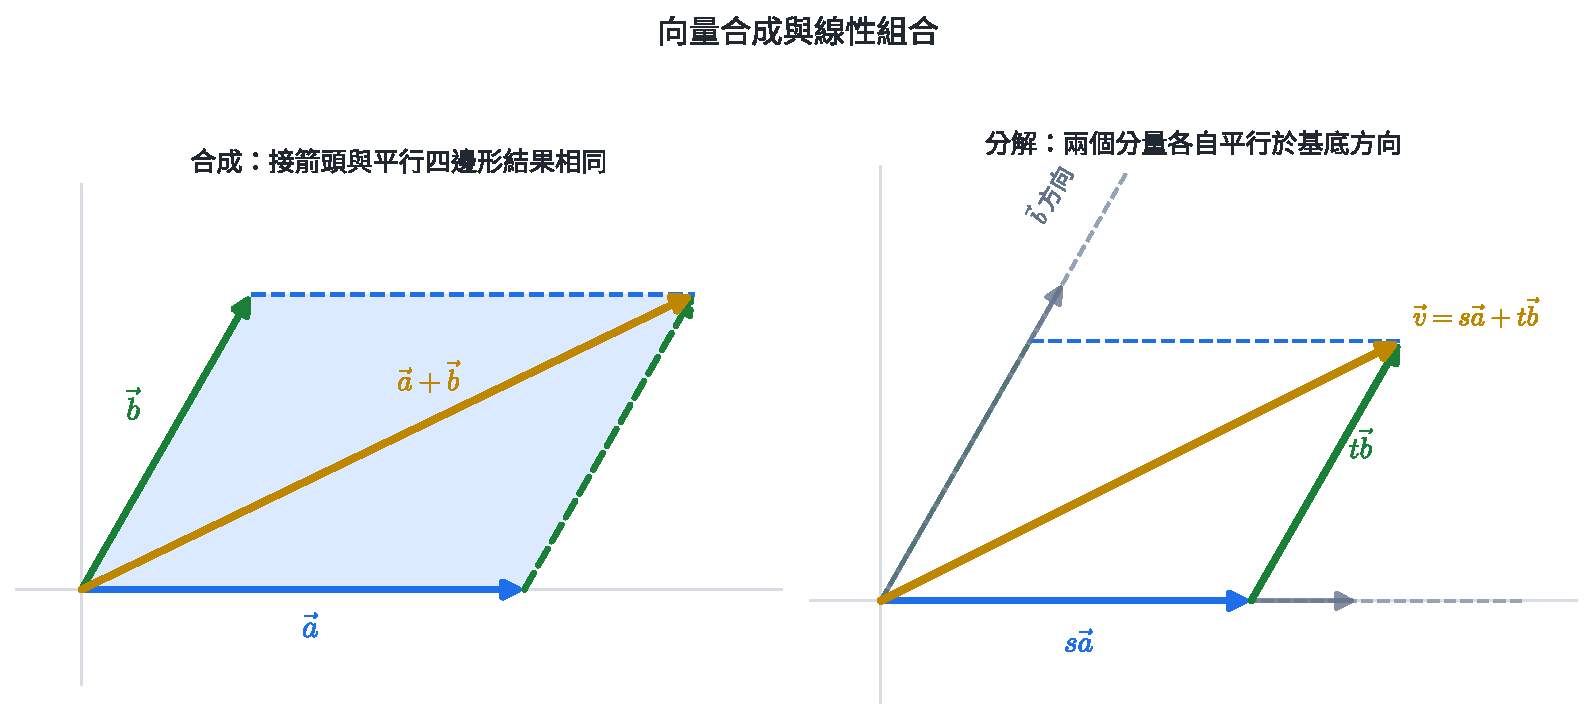
\includegraphics[width=0.95\linewidth,height=\textheight,keepaspectratio,alt={圖 1｜向量加法、分解與線性組合的幾何意義。}]{assets/數A3-3-向量合成與分解.pdf}
\caption{圖 1｜向量加法、分解與線性組合的幾何意義。}
\end{figure}

\subsection{向量如何表示並合成具有方向的量？}\label{ux5411ux91cfux5982ux4f55ux8868ux793aux4e26ux5408ux6210ux5177ux6709ux65b9ux5411ux7684ux91cf}

\textbf{大小與方向共同決定效果。} 船速 \(5\ \mathrm{m/s}\)、風速 \(5\ \mathrm{m/s}\) 若方向不同，造成的位置變化完全不同。

\textbf{坐標分量便於計算與儲存。} 分量把方向變成機器、導航與程式可儲存、可相加的數字。

\textbf{分量相加表示同時發生的效果。} 同一時間內的各方向效應一起發生，總位移的水平與鉛直分量正好各自相加。

\textbf{應用與單位條件。} 導航把自身速度與水流／風速相加；電腦圖學用位移向量移動物件；物理把力分解成容易處理的方向。相加的向量須表示同類量並使用相容單位。

\begin{HandoutWorkedExample}

\subsection{完整示範｜相對岸速度的向量合成}\label{ux5b8cux6574ux793aux7bc4ux76f8ux5c0dux5cb8ux901fux5ea6ux7684ux5411ux91cfux5408ux6210}

船相對水的速度為 \(\vec v_b=(-3,4)\ \mathrm{m/s}\)，河水速度為 \(\vec v_r=(3,0)\ \mathrm{m/s}\)。相對岸的實際速度是

\[
\vec v=\vec v_b+\vec v_r
=(-3,4)+(3,0)
=(0,4)\ \mathrm{m/s}.
\]

水平分量互相抵消，所以船會直達正對岸；過河速度為 \(4\ \mathrm{m/s}\)。而且

\[
|\vec v_b|=\sqrt{(-3)^2+4^2}=5,
\]

與船速條件一致。

\end{HandoutWorkedExample}

\subsection{1.3 平行、單位向量與線性組合}\label{ux5e73ux884cux55aeux4f4dux5411ux91cfux8207ux7ddaux6027ux7d44ux5408}

若 \(\vec a\ne\vec0\)，與它同方向的單位向量為

\[
\boxed{\frac{\vec a}{|\vec a|}}.
\]

兩個非零向量平行，等價於其中一個是另一個的實數倍：

\[
\vec a\parallel\vec b
\iff
\vec b=k\vec a.
\]

把向量寫成

\[
s\vec a+t\vec b
\]

稱為 \(\vec a,\vec b\) 的線性組合。若 \(\vec a,\vec b\) 不平行，平面上每一向量都能唯一表示成這種形式；兩個不平行向量因此可作為平面的基準方向。

\begin{HandoutWorkedExample}

\subsection{完整示範｜以線性組合表示目標向量}\label{ux5b8cux6574ux793aux7bc4ux4ee5ux7ddaux6027ux7d44ux5408ux8868ux793aux76eeux6a19ux5411ux91cf}

設

\[
\vec a=(1,1),\qquad
\vec b=(2,-1).
\]

要找 \(s,t\) 使 \(s\vec a+t\vec b=(7,1)\)，比較分量：

\[
\begin{cases}
s+2t=7,\\
s-t=1.
\end{cases}
\]

相減得 \(3t=6\)，所以 \(t=2\)、\(s=3\)。因此

\[
(7,1)=3\vec a+2\vec b.
\]

分量聯立方程就是「兩個方向各走幾倍」的操作答案。

\end{HandoutWorkedExample}

\subsection{1.4 三角不等式：合位移的長度界線}\label{ux4e09ux89d2ux4e0dux7b49ux5f0fux5408ux4f4dux79fbux7684ux9577ux5ea6ux754cux7dda}

從同一點沿 \(\vec a\) 再沿 \(\vec b\) 行走，折線路徑的總長是 \(|\vec a|+|\vec b|\)，起點到終點的直線位移是 \(|\vec a+\vec b|\)。兩點間直線最短，因此

\[
\boxed{|\vec a+\vec b|\le|\vec a|+|\vec b|}.
\]

把 \(\vec a=(\vec a-\vec b)+\vec b\) 代入同一不等式，可得

\[
\boxed{\bigl||\vec a|-|\vec b|\bigr|\le|\vec a-\vec b|}.
\]

第一式取等號時，兩段路徑沒有折角：其中一向量為零，或兩個非零向量同方向。對非零向量而言，可寫成 \(\vec a=t\vec b\) 且 \(t>0\)。

\begin{HandoutWorkedExample}

\subsection{完整示範｜只知道兩邊長也能界定合向量}\label{ux5b8cux6574ux793aux7bc4ux53eaux77e5ux9053ux5169ux908aux9577ux4e5fux80fdux754cux5b9aux5408ux5411ux91cf}

已知 \(|\vec a|=5\)、\(|\vec b|=2\)。求 \(|\vec a+\vec b|\) 的可能範圍，並說明端點何時取得。

三角不等式給上界：

\[
|\vec a+\vec b|\le5+2=7.
\]

把反向三角不等式用在 \(\vec a+\vec b=\vec a-(-\vec b)\)：

\[
|\vec a+\vec b|\ge\bigl||\vec a|-|\vec b|\bigr|=3.
\]

所以

\[
\boxed{3\le|\vec a+\vec b|\le7}.
\]

\(\vec a,\vec b\) 同方向時取 \(7\)；反方向時取 \(3\)。

\end{HandoutWorkedExample}

\subsection{\texorpdfstring{1.5 仿射組合：係數和為 \(1\) 決定直線與區域}{1.5 仿射組合：係數和為 1 決定直線與區域}}\label{ux4effux5c04ux7d44ux5408ux4fc2ux6578ux548cux70ba-1-ux6c7aux5b9aux76f4ux7ddaux8207ux5340ux57df}

設 \(A\ne B\)。直線 \(AB\) 上任一點都可寫成

\[
\boxed{
\overrightarrow{OP}
=(1-t)\overrightarrow{OA}+t\overrightarrow{OB}
},
\qquad t\in\mathbb R.
\]

兩個係數的和是 \(1\)，所以原點改變時，這個點的位置關係不會改變。參數範圍直接描述位置：

{\def\LTcaptype{none} % do not increment counter
\begin{longtable}[]{@{}ll@{}}
\toprule\noalign{}
\(t\) 的範圍 & \(P\) 的位置 \\
\midrule\noalign{}
\endhead
\bottomrule\noalign{}
\endlastfoot
\(0<t<1\) & 線段 \(AB\) 內部 \\
\(t=0,1\) & 分別為 \(A,B\) \\
\(t<0\) & \(A\) 的外側延長線 \\
\(t>1\) & \(B\) 的外側延長線 \\
\end{longtable}
}

更一般地，若

\[
\overrightarrow{OP}
=\alpha\overrightarrow{OA}+\beta\overrightarrow{OB},
\]

則 \(\alpha+\beta=1\) 一定使 \(P\) 落在直線 \(AB\) 上。若 \(O,A,B\) 不共線，\(\overrightarrow{OA},\overrightarrow{OB}\) 不平行，表示係數具有唯一性，此時還有

\[
\boxed{P\text{ 在直線 }AB\text{ 上}\iff\alpha+\beta=1}.
\]

若 \(O,A,B\) 共線，係數表示可能不唯一；此時保留「係數和為 \(1\) 足以保證在線上」，並用 \(P=(1-t)A+tB\) 表示直線上的點。

兩個獨立方向則能張成區域。若 \(\vec u,\vec v\) 不平行，

\[
\overrightarrow{OP}
=\overrightarrow{OA}+s\vec u+t\vec v,
\qquad 0\le s,t\le1,
\]

會掃過以 \(A\)、\(A+\vec u\)、\(A+\vec v\)、\(A+\vec u+\vec v\) 為頂點的平行四邊形；限制係數就是限制沿兩個方向各走多少。

\begin{HandoutWorkedExample}

\subsection{完整示範｜由參數範圍找線段上的端點}\label{ux5b8cux6574ux793aux7bc4ux7531ux53c3ux6578ux7bc4ux570dux627eux7ddaux6bb5ux4e0aux7684ux7aefux9ede}

\(A=(0,2)\)、\(B=(8,-2)\)，且

\[
P=(1-t)A+tB,
\qquad \frac14\le t\le\frac34.
\]

代入坐標：

\[
P=(8t,2-4t).
\]

參數沿固定方向連續變化，所以軌跡是 \(AB\) 的一段。兩端分別為

\[
t=\frac14:\quad P=(2,1),
\]

\[
t=\frac34:\quad P=(6,-1).
\]

故軌跡是連接 \(\boxed{(2,1)}\) 與 \(\boxed{(6,-1)}\) 的線段。

\end{HandoutWorkedExample}

\subsection{1.6 內分、外分與三角形中的分點}\label{ux5167ux5206ux5916ux5206ux8207ux4e09ux89d2ux5f62ux4e2dux7684ux5206ux9ede}

設 \(P\) 在線段 \(AB\) 上，且

\[
AP:PB=m:n.
\]

從 \(A\) 往 \(B\) 走了全程的 \(m/(m+n)\)，所以

\[
\overrightarrow{OP}
=\overrightarrow{OA}
+\frac{m}{m+n}\overrightarrow{AB}.
\]

整理後：

\[
\boxed{
\overrightarrow{OP}
=\frac{n\overrightarrow{OA}+m\overrightarrow{OB}}{m+n}
}.
\]

比例 \(m\) 會配到 \(B\)，因為 \(AP\) 越長，\(P\) 越靠近 \(B\)。

\begin{HandoutSelfCheck}

\subsection{練習｜分點}\label{ux7df4ux7fd2ux5206ux9ede}

\(A(0,3)\)、\(B(8,-1)\)，\(AP:PB=1:3\)，求 \(P\)。

\textbf{答案：}

\[
P=\frac{3A+1B}{4}
=\left(\frac{8}{4},\frac{9-1}{4}\right)
=\boxed{(2,2)}.
\]

\end{HandoutSelfCheck}

外分點可直接使用參數式 \(P=A+t(B-A)\)。例如點在 \(B\) 的外側時 \(t>1\)；先把距離比改寫成 \(t:(t-1)\)，可避免死背帶負號的公式。

三角形的重心 \(G\) 是三條中線的交點。若頂點為 \(A,B,C\)，則

\[
\boxed{
\overrightarrow{OG}
=\frac{\overrightarrow{OA}+\overrightarrow{OB}+\overrightarrow{OC}}{3}
}.
\]

若 \(AD\) 是 \(\triangle ABC\) 的內角平分線，\(D\) 在 \(BC\) 上，角平分線定理給

\[
BD:DC=AB:AC.
\]

因此角平分線上的分點可先由邊長決定比例，再套用內分公式。

\begin{HandoutWorkedExample}

\subsection{完整示範｜外分點用參數解}\label{ux5b8cux6574ux793aux7bc4ux5916ux5206ux9edeux7528ux53c3ux6578ux89e3}

\(A=(1,2)\)、\(B=(5,-2)\)，點 \(P\) 在 \(B\) 的外側，且 \(AP:PB=3:1\)。求 \(P\)。

令

\[
P=A+t(B-A),
\qquad t>1.
\]

則 \(AP=t|AB|\)、\(PB=(t-1)|AB|\)，所以

\[
\frac{t}{t-1}=3
\Longrightarrow
t=\frac32.
\]

因此

\[
P=(1,2)+\frac32(4,-4)
=\boxed{(7,-4)}.
\]

距離向量為 \(\overrightarrow{AP}=(6,-6)\)、\(\overrightarrow{PB}=(-2,2)\)；長度比確為 \(3:1\)。

\end{HandoutWorkedExample}

\begin{HandoutWorkedExample}

\subsection{完整示範｜角平分線定理接到分點公式}\label{ux5b8cux6574ux793aux7bc4ux89d2ux5e73ux5206ux7ddaux5b9aux7406ux63a5ux5230ux5206ux9edeux516cux5f0f}

在 \(\triangle ABC\) 中，\(A=(0,0)\)、\(B=(-3,4)\)、\(C=(6,8)\)。內角平分線 \(AD\) 交 \(BC\) 於 \(D\)。求 \(D\)。

先算邊長：

\[
AB=5,
\qquad
AC=10.
\]

角平分線定理給 \(BD:DC=1:2\)。因此

\[
D=\frac{2B+1C}{3}
=\frac{2(-3,4)+(6,8)}3
=\boxed{\left(0,\frac{16}{3}\right)}.
\]

\end{HandoutWorkedExample}

\begin{HandoutSelfCheck}

\subsection{節末練習｜向量、線性組合與分點}\label{ux7bc0ux672bux7df4ux7fd2ux5411ux91cfux7ddaux6027ux7d44ux5408ux8207ux5206ux9ede}

\begin{enumerate}
\def\labelenumi{\arabic{enumi}.}
\tightlist
\item
  已知 \(|\vec a|=8\)、\(|\vec b|=3\)，寫出 \(|\vec a+\vec b|\) 的可能範圍。
\item
  \(\vec a=(6,-8)\)，求與 \(\vec a\) 同方向的單位向量。
\item
  \(A=(2,-1)\)、\(B=(8,5)\)，\(P=(1-t)A+tB\)。當 \(-1\le t\le1/2\) 時，求軌跡兩端點。
\item
  若 \(\overrightarrow{OP}=k\overrightarrow{OA}+(2-k)\overrightarrow{OB}\)，判斷是否能只由此式保證 \(P\) 在直線 \(AB\) 上。
\item
  \(A=(0,0)\)、\(B=(6,3)\)，點 \(P\) 在 \(B\) 外側且 \(AP:PB=4:1\)。求 \(P\)。
\item
  三角形頂點為 \(A=(1,2)\)、\(B=(7,-1)\)、\(C=(-2,5)\)，求重心。
\end{enumerate}

\textbf{答案：}

\begin{enumerate}
\def\labelenumi{\arabic{enumi}.}
\tightlist
\item
  \(5\le|\vec a+\vec b|\le11\)。
\item
  \((3/5,-4/5)\)。
\item
  \(t=-1\) 得 \((-4,-7)\)；\(t=1/2\) 得 \((5,2)\)；軌跡為兩點間線段。
\item
  兩係數和為 \(2\)，一般不保證在直線 \(AB\) 上。
\item
  令 \(P=A+t(B-A)\)，\(t/(t-1)=4\)，得 \(t=4/3\)，所以 \(P=(8,4)\)。
\item
  \(G=((1+7-2)/3,(2-1+5)/3)=(2,2)\)。
\end{enumerate}

\end{HandoutSelfCheck}

\clearpage

\subsection{1.7 兩個係數的限制如何形成三角形}\label{ux5169ux500bux4fc2ux6578ux7684ux9650ux5236ux5982ux4f55ux5f62ux6210ux4e09ux89d2ux5f62}

平行四邊形區域使用 \(0\le s,t\le1\)，因兩個方向可各自走完整的一倍。若改成

\[
s\ge0,
\qquad
t\ge0,
\qquad
s+t\le1,
\]

兩個方向合計至多走一倍，區域會變成三角形：

\[
\overrightarrow{OP}
=\overrightarrow{OA}+s\vec u+t\vec v,
\quad
s,t\ge0,
\quad
s+t\le1
\]

的三個頂點為 \(A\)、\(A+\vec u\)、\(A+\vec v\)。

把 \(r=1-s-t\)，便有 \(r,s,t\ge0\) 且 \(r+s+t=1\)。位置向量也可寫成

\[
\overrightarrow{OP}
=r\overrightarrow{OA}
+s\overrightarrow{O(A+\vec u)}
+t\overrightarrow{O(A+\vec v)}.
\]

三個非負係數的和為 \(1\)，表示 \(P\) 是三個頂點的加權平均，因此落在三角形內部或邊界。

\begin{HandoutWorkedExample}

\subsection{完整示範｜由係數條件找區域與一次式極值}\label{ux5b8cux6574ux793aux7bc4ux7531ux4fc2ux6578ux689dux4ef6ux627eux5340ux57dfux8207ux4e00ux6b21ux5f0fux6975ux503c}

設

\[
A=(1,1),
\qquad
\vec u=(4,0),
\qquad
\vec v=(0,6),
\]

且

\[
P=A+s\vec u+t\vec v,
\qquad
s,t\ge0,
\qquad
s+t\le1.
\]

三個頂點為

\[
A=(1,1),
\quad
A+\vec u=(5,1),
\quad
A+\vec v=(1,7).
\]

\(A\) 到 \(A+\vec u\) 的水平底長為 \(4\)，\(A\) 到 \(A+\vec v\) 的鉛直高為 \(6\)，因此區域面積為

\[
\frac12\times4\times6=\boxed{12}.
\]

又

\[
P=(1+4s,1+6t),
\]

所以

\[
x+y=2+4s+6t.
\]

在 \(s,t\ge0\)、\(s+t\le1\) 下，把一單位係數放在 \(t\) 所帶來的增量 \(6\) 大於放在 \(s\) 的增量 \(4\)；最大值在 \(s=0,t=1\)：

\[
\boxed{x+y\le8},
\]

等號點為 \(\boxed{(1,7)}\)。這也等於直接比較三個頂點的一次式值。

\end{HandoutWorkedExample}

\section{2. 內積：量出方向的一致程度}\label{ux5167ux7a4dux91cfux51faux65b9ux5411ux7684ux4e00ux81f4ux7a0bux5ea6}

\subsection{2.1 夾角與兩種公式}\label{ux593eux89d2ux8207ux5169ux7a2eux516cux5f0f}

兩個非零向量平移到同一始點後，較小夾角 \(\theta\) 取在 \(0\le\theta\le\pi\)。

\[
\boxed{\vec a\cdot\vec b=|\vec a||\vec b|\cos\theta}.
\]

若 \(\vec a=(a_1,a_2)\)、\(\vec b=(b_1,b_2)\)，則

\[
\boxed{\vec a\cdot\vec b=a_1b_1+a_2b_2}.
\]

內積的結果是純量。

\begin{figure}
\centering
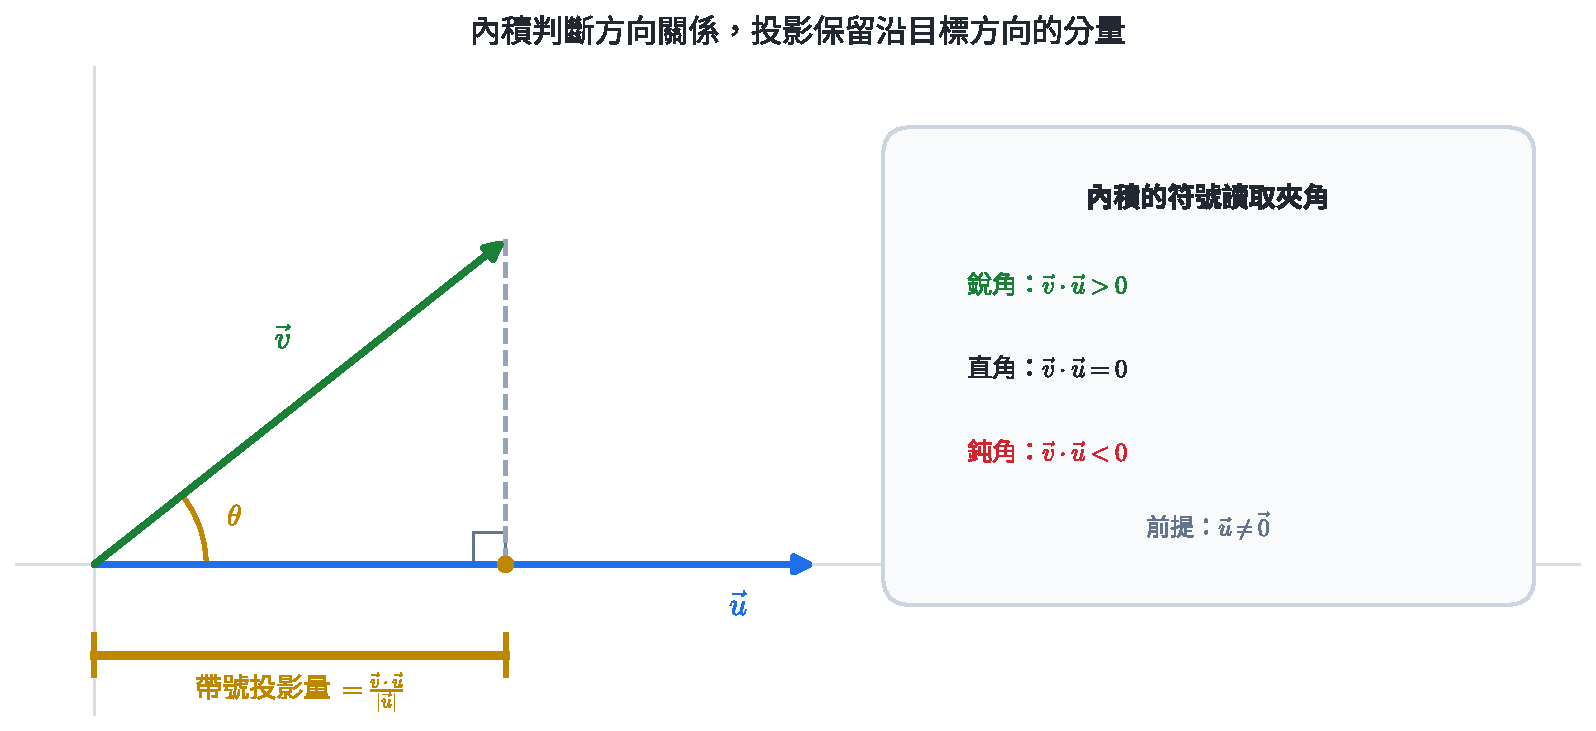
\includegraphics[width=0.92\linewidth,height=\textheight,keepaspectratio,alt={圖 2｜內積同時記錄夾角、投影與方向一致程度。}]{assets/數A3-3-內積與投影.pdf}
\caption{圖 2｜內積同時記錄夾角、投影與方向一致程度。}
\end{figure}

\subsection{幾何式與坐標式為什麼相等？}\label{ux5e7eux4f55ux5f0fux8207ux5750ux6a19ux5f0fux70baux4ec0ux9ebcux76f8ux7b49}

把 \(\vec a,\vec b\) 共起點，第三邊是 \(\vec a-\vec b\)。餘弦定理給出

\[
|\vec a-\vec b|^2
=|\vec a|^2+|\vec b|^2
-2|\vec a||\vec b|\cos\theta.
\]

用坐標直接展開同一個長度：

\[
\begin{aligned}
|\vec a-\vec b|^2
&=(a_1-b_1)^2+(a_2-b_2)^2\\
&=|\vec a|^2+|\vec b|^2
-2(a_1b_1+a_2b_2).
\end{aligned}
\]

兩式在算同一段長度，對照後便得到

\[
a_1b_1+a_2b_2=|\vec a||\vec b|\cos\theta.
\]

內積把三種幾何問題化成代數：

\[
\cos\theta=\frac{\vec a\cdot\vec b}{|\vec a||\vec b|},
\]

\[
\vec a\perp\vec b
\iff
\vec a\cdot\vec b=0
\quad(\vec a,\vec b\ne\vec0),
\]

在 \(\vec a,\vec b\) 皆為非零向量時，內積為正、零、負，分別對應銳角、直角、鈍角。

\begin{HandoutWorkedExample}

\subsection{完整示範｜由坐標求夾角}\label{ux5b8cux6574ux793aux7bc4ux7531ux5750ux6a19ux6c42ux593eux89d2}

設

\[
\vec a=(1,\sqrt3),
\qquad
\vec b=(2,0).
\]

先算內積與長度：

\[
\vec a\cdot\vec b=2,
\qquad
|\vec a|=2,
\qquad
|\vec b|=2.
\]

因此

\[
\cos\theta
=\frac{\vec a\cdot\vec b}{|\vec a||\vec b|}
=\frac{2}{4}
=\frac12.
\]

較小夾角 \(0\le\theta\le\pi\)，故

\[
\boxed{\theta=60^\circ}.
\]

\end{HandoutWorkedExample}

\subsection{2.2 運算性質與長度}\label{ux904bux7b97ux6027ux8ceaux8207ux9577ux5ea6}

\[
\vec a\cdot\vec b=\vec b\cdot\vec a,
\]

\[
\vec a\cdot(\vec b+\vec c)
=\vec a\cdot\vec b+\vec a\cdot\vec c,
\]

\[
(k\vec a)\cdot\vec b
=k(\vec a\cdot\vec b),
\]

\[
\vec a\cdot\vec a=|\vec a|^2.
\]

因此

\[
|\vec a+\vec b|^2
=|\vec a|^2+2\vec a\cdot\vec b+|\vec b|^2,
\]

這是向量版的平方公式。

\begin{HandoutWorkedExample}

\subsection{完整示範｜用內積求線性組合的長度}\label{ux5b8cux6574ux793aux7bc4ux7528ux5167ux7a4dux6c42ux7ddaux6027ux7d44ux5408ux7684ux9577ux5ea6}

已知 \(|\vec a|=2\)、\(|\vec b|=3\)，夾角為 \(60^\circ\)。求 \(|2\vec a-\vec b|\)。

先求

\[
\vec a\cdot\vec b
=2\cdot3\cdot\cos60^\circ
=3.
\]

再平方：

\[
\begin{aligned}
|2\vec a-\vec b|^2
&=(2\vec a-\vec b)\cdot(2\vec a-\vec b)\\
&=4|\vec a|^2-4\vec a\cdot\vec b+|\vec b|^2\\
&=16-12+9=13.
\end{aligned}
\]

故 \(\boxed{|2\vec a-\vec b|=\sqrt{13}}\)。

\end{HandoutWorkedExample}

\subsection{2.3 正射影：只留下沿目標方向的部分}\label{ux6b63ux5c04ux5f71ux53eaux7559ux4e0bux6cbfux76eeux6a19ux65b9ux5411ux7684ux90e8ux5206}

設 \(\vec u\ne\vec0\)。\(\vec v\) 在 \(\vec u\) 方向上的：

\textbf{帶號投影量}

\[
\boxed{\frac{\vec v\cdot\vec u}{|\vec u|}}
\]

\textbf{投影向量}

\[
\boxed{
\operatorname{proj}_{\vec u}\vec v
=\frac{\vec v\cdot\vec u}{|\vec u|^2}\vec u
}.
\]

投影量可為負，表示投影落在 \(\vec u\) 的反方向；投影向量一定平行於 \(\vec u\)。

\subsection{內積如何量化方向一致性？}\label{ux5167ux7a4dux5982ux4f55ux91cfux5316ux65b9ux5411ux4e00ux81f4ux6027}

\textbf{方向比例。} \(\cos\theta\) 取出「沿著另一方向」的比例；垂直時比例為 \(0\)，反向時為負。

\textbf{尺度。} 一個長度提供被投影的量，另一個長度讓結果隨兩向量尺度一起變化。

\textbf{應用與前提。} 當力在所考慮位移中可視為恆定時，功 \(W=\vec F\cdot\vec s\) 只計算沿位移方向的力；搜尋系統中的簡化餘弦相似度（要求 \(\vec a,\vec b\) 皆為非零向量）

\[
\frac{\vec a\cdot\vec b}{|\vec a||\vec b|}
\]

比較兩組特徵的方向相似程度。實際辨識結果還取決於特徵建模、資料品質與判定門檻。

\begin{HandoutSelfCheck}

\subsection{練習｜內積與投影}\label{ux7df4ux7fd2ux5167ux7a4dux8207ux6295ux5f71}

\(\vec u=(3,4)\)、\(\vec v=(4,-3)\)。兩向量是否垂直？\(\vec v\) 在 \(\vec u\) 上的投影向量為何？

\textbf{答案：}\(\vec u\cdot\vec v=12-12=0\)，所以垂直；投影向量為 \(\vec0\)。

\end{HandoutSelfCheck}

\begin{HandoutWorkedExample}

\subsection{完整示範｜把向量分成平行與垂直兩部分}\label{ux5b8cux6574ux793aux7bc4ux628aux5411ux91cfux5206ux6210ux5e73ux884cux8207ux5782ux76f4ux5169ux90e8ux5206}

將 \(\vec v=(5,4)\) 分解成平行於 \(\vec u=(2,1)\) 的部分與垂直於 \(\vec u\) 的部分。

先算

\[
\vec v\cdot\vec u=14,
\qquad
|\vec u|^2=5.
\]

平行部分為

\[
\vec v_{\parallel}
=\operatorname{proj}_{\vec u}\vec v
=\frac{14}{5}(2,1)
=\boxed{\left(\frac{28}{5},\frac{14}{5}\right)}.
\]

垂直部分為

\[
\begin{aligned}
\vec v_{\perp}
&=\vec v-\vec v_{\parallel}\\
&=\left(5,4\right)-\left(\frac{28}{5},\frac{14}{5}\right)\\
&=\boxed{\left(-\frac35,\frac65\right)}.
\end{aligned}
\]

驗算：

\[
\vec v_{\perp}\cdot\vec u
=-\frac35(2)+\frac65(1)=0,
\]

所以第二部分確實垂直於 \(\vec u\)。

\end{HandoutWorkedExample}

\subsection{2.4 柯西不等式與極值}\label{ux67efux897fux4e0dux7b49ux5f0fux8207ux6975ux503c}

由

\[
\vec a\cdot\vec b=|\vec a||\vec b|\cos\theta
\]

及 \(|\cos\theta|\le1\)：

\[
\boxed{
|\vec a\cdot\vec b|
\le|\vec a||\vec b|
}
\]

或

\[
\boxed{
(a_1b_1+a_2b_2)^2
\le(a_1^2+a_2^2)(b_1^2+b_2^2)
}.
\]

等號成立當且僅當其中一個向量是另一個的實數倍；兩向量皆非零時，就是彼此平行。若其中一個是零向量，等號也成立。

看到「平方和固定，求一次式極值」，可把一次式配成內積；等號條件則告訴我們極值在哪裡取得。

\begin{HandoutWorkedExample}

\subsection{完整示範｜柯西不等式同時給極值與等號位置}\label{ux5b8cux6574ux793aux7bc4ux67efux897fux4e0dux7b49ux5f0fux540cux6642ux7d66ux6975ux503cux8207ux7b49ux865fux4f4dux7f6e}

已知 \(x^2+y^2\le100\)，求 \(3x+4y\) 的最大值與最小值。

把一次式寫成內積：

\[
3x+4y=(3,4)\cdot(x,y).
\]

由柯西不等式，

\[
|3x+4y|
\le\sqrt{3^2+4^2}\sqrt{x^2+y^2}
\le5\cdot10=50.
\]

最大值 \(50\) 在 \((x,y)\) 與 \((3,4)\) 同方向、且長度為 \(10\) 時取得：

\[
(x,y)=2(3,4)=(6,8).
\]

最小值 \(-50\) 在反方向時取得：

\[
(x,y)=(-6,-8).
\]

故

\[
\boxed{-50\le3x+4y\le50}.
\]

\end{HandoutWorkedExample}

\subsection{2.5 直線的法向量}\label{ux76f4ux7ddaux7684ux6cd5ux5411ux91cf}

若 \((a,b)\ne(0,0)\)，方程

\[
L:ax+by+c=0
\]

才確實表示一條直線。它的方向向量可取 \((b,-a)\)，所以垂直於直線的法向量可取

\[
\boxed{\vec n=(a,b)}.
\]

兩直線的夾角可改成其方向向量或法向量的夾角。點 \(P(x_0,y_0)\) 到直線的距離，也可視為某段位移在法向量上的投影：

\[
\boxed{
d=\frac{|ax_0+by_0+c|}{\sqrt{a^2+b^2}}
}.
\]

分母是非零法向量的長度。公式要求 \((a,b)\ne(0,0)\)；\(a=b=0\) 時，方程與分母都退化。

\subsection{點線距離與垂足公式的投影來源}\label{ux9edeux7ddaux8dddux96e2ux8207ux5782ux8db3ux516cux5f0fux7684ux6295ux5f71ux4f86ux6e90}

在直線 \(L:ax+by+c=0\) 上任取一點 \(Q=(x_1,y_1)\)，則

\[
ax_1+by_1+c=0.
\]

對 \(P=(x_0,y_0)\)，位移 \(\overrightarrow{QP}\) 在法向量 \(\vec n=(a,b)\) 上的帶號投影量為

\[
\frac{\overrightarrow{QP}\cdot\vec n}{|\vec n|}
=\frac{a(x_0-x_1)+b(y_0-y_1)}{\sqrt{a^2+b^2}}.
\]

利用 \(ax_1+by_1=-c\)，分子化成 \(ax_0+by_0+c\)。取絕對值便得到點線距離公式。

垂足 \(H\) 則是從 \(P\) 沿法向量退回直線。設

\[
H=P-\lambda(a,b).
\]

把 \(H\) 代入直線方程，可得

\[
\lambda=\frac{ax_0+by_0+c}{a^2+b^2}.
\]

因此

\[
\boxed{
H=(x_0,y_0)
-\frac{ax_0+by_0+c}{a^2+b^2}(a,b)
}.
\]

\begin{HandoutWorkedExample}

\subsection{完整示範｜求垂足並用方程驗證}\label{ux5b8cux6574ux793aux7bc4ux6c42ux5782ux8db3ux4e26ux7528ux65b9ux7a0bux9a57ux8b49}

求點 \(P=(4,0)\) 到直線

\[
L:2x-y+1=0
\]

的垂足與距離。

這裡 \((a,b,c)=(2,-1,1)\)，所以

\[
ax_0+by_0+c=2(4)-0+1=9,
\qquad
a^2+b^2=5.
\]

垂足

\[
\begin{aligned}
H
&=(4,0)-\frac95(2,-1)\\
&=\boxed{\left(\frac25,\frac95\right)}.
\end{aligned}
\]

代入直線：

\[
2\left(\frac25\right)-\frac95+1=0,
\]

所以 \(H\) 確實在 \(L\) 上。距離為

\[
PH=\frac{|9|}{\sqrt5}
=\boxed{\frac{9\sqrt5}{5}}.
\]

\end{HandoutWorkedExample}

\begin{HandoutWorkedExample}

\subsection{完整示範｜由法向量求平行線、垂直線與點線距離}\label{ux5b8cux6574ux793aux7bc4ux7531ux6cd5ux5411ux91cfux6c42ux5e73ux884cux7ddaux5782ux76f4ux7ddaux8207ux9edeux7ddaux8dddux96e2}

給定

\[
L:3x-4y+8=0
\]

與點 \(P=(2,5)\)。

\(L\) 的法向量可取 \((3,-4)\)，方向向量可取 \((4,3)\)。

通過 \(P\) 且平行於 \(L\) 的直線沿用同一法向量：

\[
3(x-2)-4(y-5)=0
\Longrightarrow
\boxed{3x-4y+14=0}.
\]

通過 \(P\) 且垂直於 \(L\) 的直線可用 \((4,3)\) 作法向量：

\[
4(x-2)+3(y-5)=0
\Longrightarrow
\boxed{4x+3y-23=0}.
\]

點到 \(L\) 的距離為

\[
d=\frac{|3(2)-4(5)+8|}{\sqrt{3^2+(-4)^2}}
=\frac6{5}.
\]

所以 \(\boxed{d=6/5}\)。

\end{HandoutWorkedExample}

\begin{HandoutSelfCheck}

\subsection{節末練習｜內積、投影、極值與直線}\label{ux7bc0ux672bux7df4ux7fd2ux5167ux7a4dux6295ux5f71ux6975ux503cux8207ux76f4ux7dda}

\begin{enumerate}
\def\labelenumi{\arabic{enumi}.}
\tightlist
\item
  求 \(\vec a=(3,1)\)、\(\vec b=(-1,2)\) 的夾角 cosine，並判斷是銳角或鈍角。
\item
  求 \(k\)，使 \((k,3)\) 與 \((2,-4)\) 垂直。
\item
  求 \(\vec v=(4,5)\) 在 \(\vec u=(1,2)\) 上的投影向量。
\item
  已知 \(x^2+y^2=25\)，求 \(4x-3y\) 的最大值及等號位置。
\item
  求點 \((1,-2)\) 到直線 \(2x+y-7=0\) 的距離。
\item
  求通過 \((3,1)\) 且垂直於 \(x+2y-5=0\) 的直線方程。
\end{enumerate}

\textbf{答案：}

\begin{enumerate}
\def\labelenumi{\arabic{enumi}.}
\tightlist
\item
  \(\cos\theta=(-3+2)/(\sqrt{10}\sqrt5)=-1/\sqrt{50}\)，所以是鈍角。
\item
  \(2k-12=0\)，故 \(k=6\)。
\item
  \((\vec v\cdot\vec u/|\vec u|^2)\vec u=(14/5)(1,2)=(14/5,28/5)\)。
\item
  最大值 \(25\)；在 \((x,y)=(4,-3)\) 取得。
\item
  \(|2(1)+(-2)-7|/\sqrt5=7/\sqrt5=7\sqrt5/5\)。
\item
  原直線方向向量可取 \((2,-1)\)；所求直線以 \((2,-1)\) 為法向量：\(2(x-3)-(y-1)=0\)，即 \(2x-y-5=0\)。
\end{enumerate}

\end{HandoutSelfCheck}

\section{3. 二階行列式：面積、方向與聯立方程}\label{ux4e8cux968eux884cux5217ux5f0fux9762ux7a4dux65b9ux5411ux8207ux806fux7acbux65b9ux7a0b}

\subsection{3.1 面積與定向}\label{ux9762ux7a4dux8207ux5b9aux5411}

設

\[
\vec a=(a_1,a_2),\qquad
\vec b=(b_1,b_2).
\]

定義二階行列式

\[
\det(\vec a,\vec b)
=
\begin{vmatrix}
a_1&b_1\\
a_2&b_2
\end{vmatrix}
=a_1b_2-a_2b_1.
\]

由 \(\vec a,\vec b\) 張成的平行四邊形面積：

\[
\boxed{
A_{\text{平行四邊形}}
=|\det(\vec a,\vec b)|
}.
\]

由同一頂點出發的兩邊所成三角形面積：

\[
\boxed{
A_{\triangle}
=\frac12|\det(\vec a,\vec b)|
}.
\]

\begin{figure}
\centering
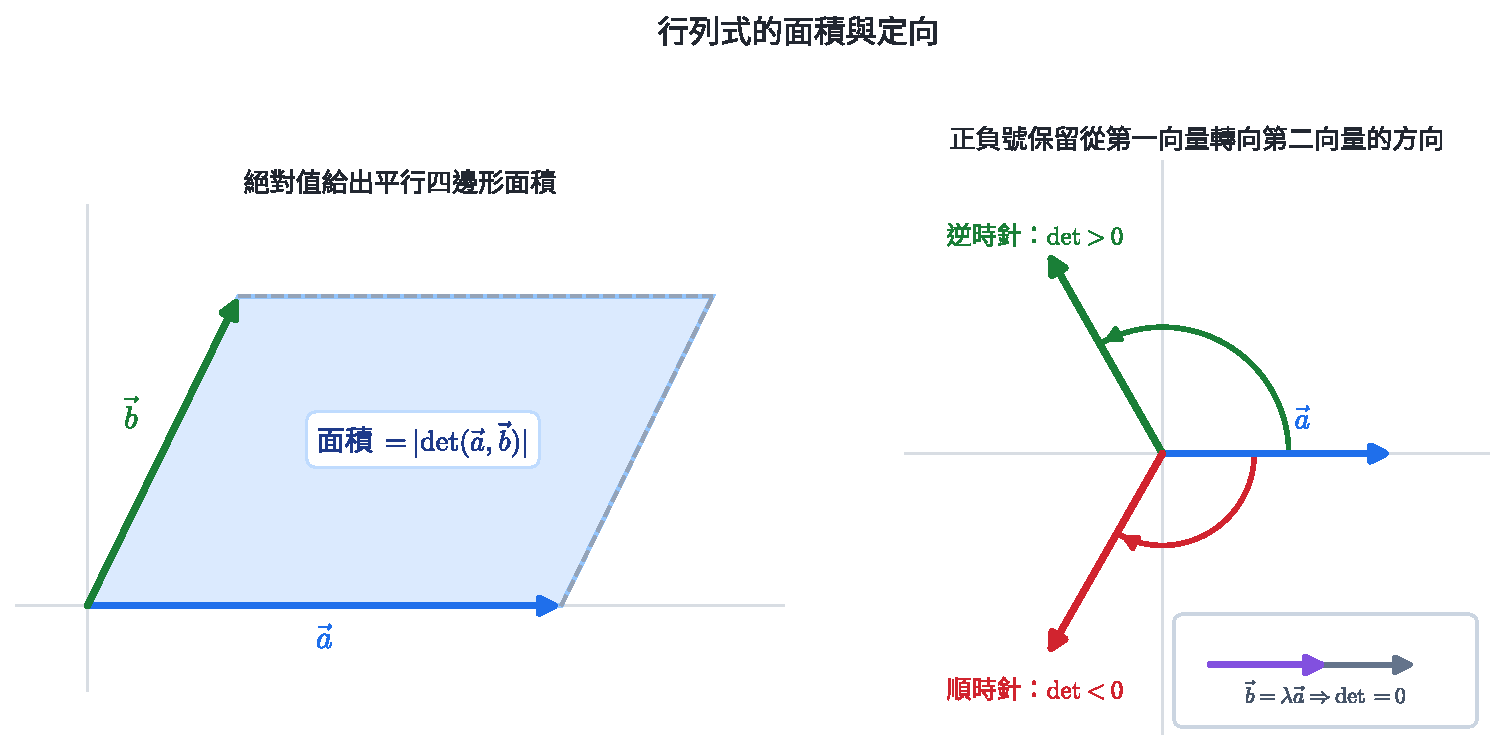
\includegraphics[width=0.92\linewidth,height=\textheight,keepaspectratio,alt={圖 3｜行列式的絕對值是面積，正負號記錄轉向。}]{assets/數A3-3-行列式面積與定向.pdf}
\caption{圖 3｜行列式的絕對值是面積，正負號記錄轉向。}
\end{figure}

\subsection{\texorpdfstring{為什麼 \(a_1b_2-a_2b_1\) 會給出面積？}{為什麼 a\_1b\_2-a\_2b\_1 會給出面積？}}\label{ux70baux4ec0ux9ebc-a_1b_2-a_2b_1-ux6703ux7d66ux51faux9762ux7a4d}

平行四邊形面積為

\[
A=|\vec a||\vec b||\sin\theta|.
\]

又

\[
\begin{aligned}
A^2
&=|\vec a|^2|\vec b|^2-(\vec a\cdot\vec b)^2\\
&=(a_1^2+a_2^2)(b_1^2+b_2^2)
-(a_1b_1+a_2b_2)^2\\
&=(a_1b_2-a_2b_1)^2.
\end{aligned}
\]

因面積非負，開根號後取絕對值。

不取絕對值時，行列式的正負還有幾何意義：

\begin{itemize}
\tightlist
\item
  \(\det(\vec a,\vec b)>0\)：從 \(\vec a\) 轉向 \(\vec b\) 是逆時針；
\item
  \(\det(\vec a,\vec b)<0\)：是順時針；
\item
  \(\det(\vec a,\vec b)=0\)：兩向量線性相依，張成的圖形退化且面積為 \(0\)；若兩者都非零，才可說它們平行。
\end{itemize}

\begin{HandoutWorkedExample}

\subsection{完整示範｜三點面積與排列方向一起判斷}\label{ux5b8cux6574ux793aux7bc4ux4e09ux9edeux9762ux7a4dux8207ux6392ux5217ux65b9ux5411ux4e00ux8d77ux5224ux65b7}

\(A=(-1,2)\)、\(B=(4,3)\)、\(C=(2,7)\)。求 \(\triangle ABC\) 面積，並判斷 \(A\to B\to C\) 的轉向。

從同一頂點 \(A\) 出發：

\[
\overrightarrow{AB}=(5,1),
\qquad
\overrightarrow{AC}=(3,5).
\]

行列式為

\[
\det(\overrightarrow{AB},\overrightarrow{AC})
=5\cdot5-1\cdot3=22.
\]

所以

\[
A_{\triangle ABC}=\frac12|22|=\boxed{11}.
\]

行列式為正，因此從 \(\overrightarrow{AB}\) 轉到 \(\overrightarrow{AC}\) 是逆時針；\(A\to B\to C\) 為左轉。

\end{HandoutWorkedExample}

\subsection{行列式為什麼保留正負？}\label{ux884cux5217ux5f0fux70baux4ec0ux9ebcux4fddux7559ux6b63ux8ca0}

\textbf{幾何面積。} 幾何面積取行列式的絕對值。

\textbf{定向資訊。} 正負號保留頂點的排列方向；交換兩向量，旋轉方向反轉，行列式也變號。

\textbf{應用與範圍。} 地圖與電腦圖學可用行列式符號判斷三點是左轉、右轉或共線；三角網格也用一致定向避免把面翻反。這裡只使用二維幾何判斷，不延伸到三維外積。

\subsection{3.2 行列式的基本性質}\label{ux884cux5217ux5f0fux7684ux57faux672cux6027ux8cea}

由 \(ad-bc\) 直接展開可得：

\begin{enumerate}
\def\labelenumi{\arabic{enumi}.}
\tightlist
\item
  交換兩行或兩列，行列式變號；
\item
  某一行或列乘 \(k\)，行列式也乘 \(k\)；
\item
  某一行加上另一行的 \(k\) 倍，行列式不變；
\item
  兩行或兩列成比例時，行列式為 \(0\)。
\end{enumerate}

這些性質可以簡化計算；二階情形也可直接展開 \(ad-bc\) 驗證。

\begin{HandoutWorkedExample}

\subsection{完整示範｜用加倍數性質保留行列式}\label{ux5b8cux6574ux793aux7bc4ux7528ux52a0ux500dux6578ux6027ux8ceaux4fddux7559ux884cux5217ux5f0f}

計算

\[
\begin{vmatrix}
2&5\\
3&7
\end{vmatrix}.
\]

第二欄減去第一欄的 \(2\) 倍，行列式不變：

\[
\begin{vmatrix}
2&5\\
3&7
\end{vmatrix}
=
\begin{vmatrix}
2&1\\
3&1
\end{vmatrix}
=2-3
=\boxed{-1}.
\]

直接展開原式也得 \(2\cdot7-3\cdot5=-1\)。欄運算的作用是讓數字變簡單，行列式值仍由同一個面積倍率決定。

\end{HandoutWorkedExample}

\begin{HandoutWorkedExample}

\subsection{完整示範｜沿底邊平移頂點，面積保持不變}\label{ux5b8cux6574ux793aux7bc4ux6cbfux5e95ux908aux5e73ux79fbux9802ux9edeux9762ux7a4dux4fddux6301ux4e0dux8b8a}

令

\[
A=(0,0),
\qquad
B=(6,0),
\qquad
C=(t,4).
\]

雖然 \(C\) 的水平位置隨 \(t\) 改變，三角形底 \(AB\) 與高仍分別為 \(6\)、\(4\)。用行列式計算：

\[
\overrightarrow{AB}=(6,0),
\qquad
\overrightarrow{AC}=(t,4),
\]

\[
\det(\overrightarrow{AB},\overrightarrow{AC})
=6\cdot4-0\cdot t=24.
\]

所以對所有實數 \(t\)，

\[
\boxed{A_{\triangle ABC}=12}.
\]

把 \(C\) 沿著與底邊平行的方向平移，相當於在第二欄加上第一欄的某個倍數；這正是行列式不變的欄運算。幾何上的「同底等高」與代數性質是同一件事。

\end{HandoutWorkedExample}

\begin{HandoutSelfCheck}

\subsection{練習｜面積與定向}\label{ux7df4ux7fd2ux9762ux7a4dux8207ux5b9aux5411}

\(\vec a=(4,1)\)、\(\vec b=(2,5)\)。求平行四邊形面積，並判斷從 \(\vec a\) 到 \(\vec b\) 的轉向。

\textbf{答案：}

\[
\det(\vec a,\vec b)=4\cdot5-1\cdot2=18>0.
\]

面積為 \(\boxed{18}\)，方向為逆時針。

\end{HandoutSelfCheck}

\subsection{3.3 二階方陣、矩陣乘向量與克拉瑪公式}\label{ux4e8cux968eux65b9ux9663ux77e9ux9663ux4e58ux5411ux91cfux8207ux514bux62c9ux746aux516cux5f0f}

考慮二元一次方程組

\[
\begin{cases}
a_1x+b_1y=c_1,\\
a_2x+b_2y=c_2.
\end{cases}
\]

由 \(2\) 列、\(2\) 欄排成的數表稱為\textbf{二階方陣}：

\[
A=
\begin{pmatrix}
a_1&b_1\\
a_2&b_2
\end{pmatrix}.
\]

在上述方程組中，\(A\) 收集未知數 \(x,y\) 的係數，稱為方程組的\textbf{係數矩陣}。令

\[
\mathbf{x}=\begin{pmatrix}x\\y\end{pmatrix},
\qquad
\mathbf{c}=\begin{pmatrix}c_1\\c_2\end{pmatrix}.
\]

二階方陣乘直行向量的定義為

\[
\boxed{
\begin{pmatrix}
a_1&b_1\\
a_2&b_2
\end{pmatrix}
\begin{pmatrix}x\\y\end{pmatrix}
=
\begin{pmatrix}
a_1x+b_1y\\
a_2x+b_2y
\end{pmatrix}}
\]

因此原方程組可簡寫為

\[
A\mathbf{x}=\mathbf{c}.
\]

乘積的第一個分量由第一列與 \((x,y)\) 對應相乘後相加，第二個分量由第二列以同樣規則得到。若改從欄向量觀察，矩陣乘法等於

\[
A\mathbf{x}
=x\begin{pmatrix}a_1\\a_2\end{pmatrix}
+y\begin{pmatrix}b_1\\b_2\end{pmatrix};
\]

解方程組就是找出兩個係數，使係數矩陣的兩欄線性組合成目標向量 \(\mathbf{c}\)。

令

\[
\Delta=
\begin{vmatrix}
a_1&b_1\\
a_2&b_2
\end{vmatrix},
\quad
\Delta_x=
\begin{vmatrix}
c_1&b_1\\
c_2&b_2
\end{vmatrix},
\quad
\Delta_y=
\begin{vmatrix}
a_1&c_1\\
a_2&c_2
\end{vmatrix}.
\]

若 \(\Delta\ne0\)，方程組恰有一組解：

\[
\boxed{x=\frac{\Delta_x}{\Delta},\qquad
y=\frac{\Delta_y}{\Delta}}.
\]

\begin{figure}
\centering
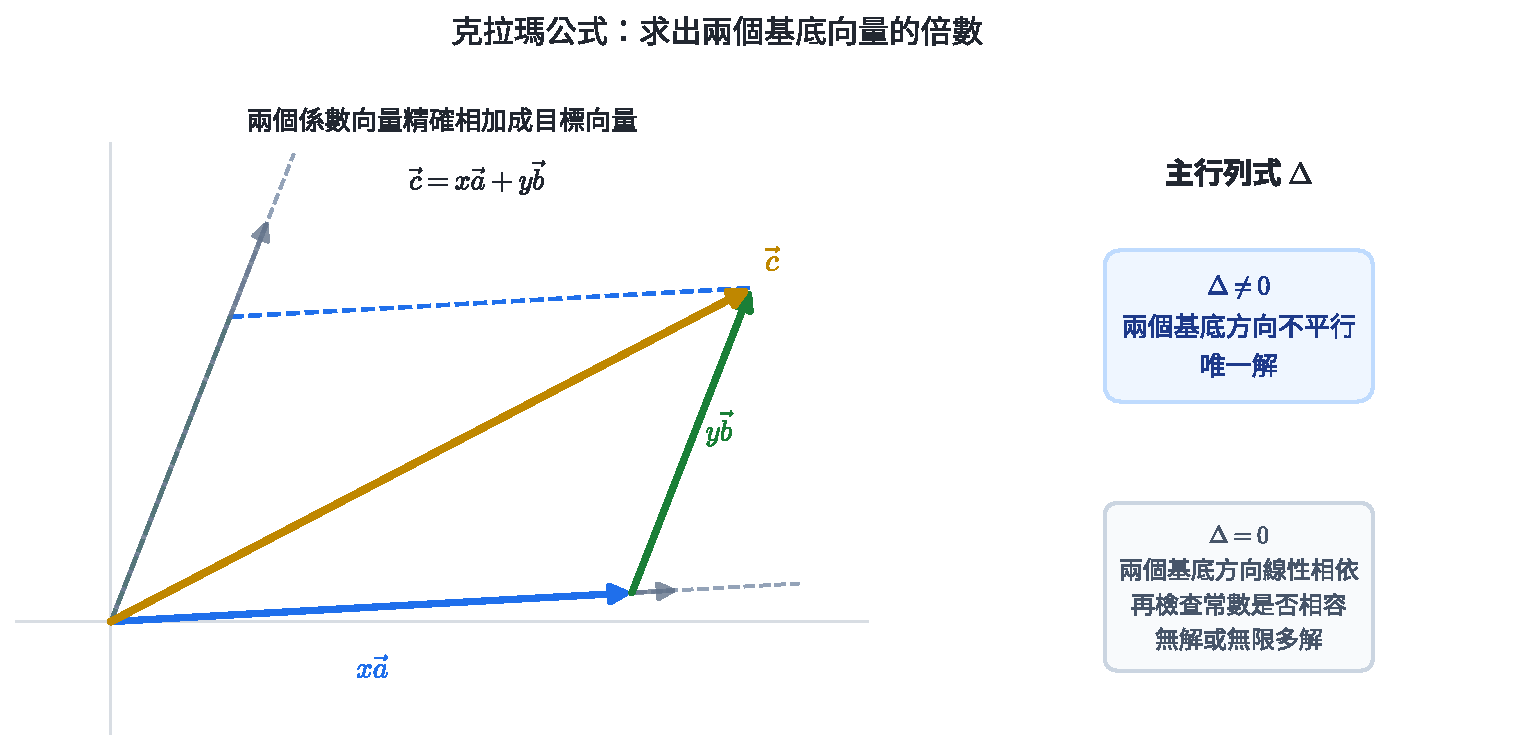
\includegraphics[width=0.92\linewidth,height=\textheight,keepaspectratio,alt={圖 4｜克拉瑪公式把目標向量分解成兩個基底向量。}]{assets/數A3-3-克拉瑪線性組合.pdf}
\caption{圖 4｜克拉瑪公式把目標向量分解成兩個基底向量。}
\end{figure}

\subsection{克拉瑪公式如何由行列式抽出係數}\label{ux514bux62c9ux746aux516cux5f0fux5982ux4f55ux7531ux884cux5217ux5f0fux62bdux51faux4fc2ux6578}

把三個直行向量記為

\[
\vec a=\begin{pmatrix}a_1\\a_2\end{pmatrix},
\quad
\vec b=\begin{pmatrix}b_1\\b_2\end{pmatrix},
\quad
\vec c=\begin{pmatrix}c_1\\c_2\end{pmatrix}.
\]

方程組就是

\[
\vec c=x\vec a+y\vec b.
\]

在兩邊的第二欄都放 \(\vec b\)，並取行列式：

\[
\begin{aligned}
\det(\vec c,\vec b)
&=\det(x\vec a+y\vec b,\vec b)\\
&=x\det(\vec a,\vec b)+y\det(\vec b,\vec b)\\
&=x\Delta.
\end{aligned}
\]

因 \(\det(\vec b,\vec b)=0\)，\(y\) 項被消去，所以 \(\Delta_x=x\Delta\)。同理，

\[
\det(\vec a,\vec c)=y\Delta,
\]

即 \(\Delta_y=y\Delta\)。當 \(\Delta\ne0\) 時可相除，得到

\[
x=\frac{\Delta_x}{\Delta},
\qquad
y=\frac{\Delta_y}{\Delta}.
\]

這個推導使用行列式對每一欄的分配律；二階情形可直接展開 \(ad-bc\) 驗證。

\(\Delta\ne0\) 表示兩個係數向量線性獨立，能唯一張成目標；\(\Delta=0\) 表示它們線性相依，這時需再看常數是否相容。以下分類假設兩個方程都確實表示直線，也就是每一式的 \(x,y\) 係數不全為 \(0\)：

\begin{itemize}
\tightlist
\item
  \(\Delta=0\)，但 \(\Delta_x\) 或 \(\Delta_y\) 非零：無解，兩直線平行；
\item
  \(\Delta=\Delta_x=\Delta_y=0\)：無限多解，兩直線重合。
\end{itemize}

\begin{HandoutWorkedExample}

\subsection{完整示範｜用克拉瑪公式解二元一次方程組}\label{ux5b8cux6574ux793aux7bc4ux7528ux514bux62c9ux746aux516cux5f0fux89e3ux4e8cux5143ux4e00ux6b21ux65b9ux7a0bux7d44}

解

\[
\begin{cases}
3x+2y=7,\\
x-y=4.
\end{cases}
\]

三個行列式為

\[
\Delta=
\begin{vmatrix}
3&2\\
1&-1
\end{vmatrix}
=-3-2=-5,
\]

\[
\Delta_x=
\begin{vmatrix}
7&2\\
4&-1
\end{vmatrix}
=-7-8=-15,
\]

\[
\Delta_y=
\begin{vmatrix}
3&7\\
1&4
\end{vmatrix}
=12-7=5.
\]

因 \(\Delta\ne0\)，有唯一解：

\[
\boxed{x=\frac{-15}{-5}=3,
\qquad
y=\frac5{-5}=-1}.
\]

代回第一式得 \(9-2=7\)，第二式得 \(3-(-1)=4\)。

\end{HandoutWorkedExample}

\begin{HandoutWorkedExample}

\subsection{完整示範｜用兩項生產紀錄判斷資料是否足以還原工時}\label{ux5b8cux6574ux793aux7bc4ux7528ux5169ux9805ux751fux7522ux7d00ux9304ux5224ux65b7ux8cc7ux6599ux662fux5426ux8db3ux4ee5ux9084ux539fux5de5ux6642}

某工廠有甲、乙兩條產線。甲線每小時加工 \(2\) 公斤原料並耗電 \(1\) 度，乙線每小時加工 \(4\) 公斤原料並耗電 \(2\) 度。令 \(x,y\) 分別為兩條產線的運轉時數；工時可連續計量，且 \(x,y\ge0\)。

這個判別可檢查量測紀錄的一致性：兩個讀值若來自相同比例的量測機制，就無法單獨辨識兩個未知來源。

係數矩陣為

\[
A=
\begin{pmatrix}
2&4\\
1&2
\end{pmatrix},
\qquad
\Delta=2\cdot2-1\cdot4=0.
\]

兩欄成比例，表示兩條產線的「加工量與耗電量之比」相同；兩項總量紀錄可能只是同一項資訊的倍數，未必能分辨各線工時。

\textbf{紀錄一：總加工量 \(20\) 公斤、總耗電量 \(10\) 度。} 方程組為

\[
\begin{cases}
2x+4y=20,\\
x+2y=10.
\end{cases}
\]

此時

\[
\Delta_x=
\begin{vmatrix}
20&4\\
10&2
\end{vmatrix}=0,
\qquad
\Delta_y=
\begin{vmatrix}
2&20\\
1&10
\end{vmatrix}=0.
\]

第一式正好是第二式的 \(2\) 倍，兩式共同留下

\[
x+2y=10.
\]

令 \(y=t\)，則 \(x=10-2t\)。配合 \(x,y\ge0\)，得到

\[
\boxed{(x,y)=(10-2t,t),\qquad 0\le t\le5}.
\]

可行解包含 \((10,0)\)、\((6,2)\)、\((0,5)\) 等無限多組。兩份紀錄彼此相容，卻沒有提供足以分開兩條產線的獨立資訊，因此無法唯一還原工時。

\textbf{紀錄二：總加工量 \(20\) 公斤、總耗電量 \(9\) 度。} 方程組改為

\[
\begin{cases}
2x+4y=20,\\
x+2y=9.
\end{cases}
\]

係數矩陣不變，所以 \(\Delta=0\)；進一步計算

\[
\Delta_x=
\begin{vmatrix}
20&4\\
9&2
\end{vmatrix}=4,
\qquad
\Delta_y=
\begin{vmatrix}
2&20\\
1&9
\end{vmatrix}=-2.
\]

任一替換行列式非零即表示常數與原本的比例關係不相容。把第二式乘以 \(2\) 會得到 \(2x+4y=18\)，與第一式要求的 \(2x+4y=20\) 衝突，所以方程組無解。

\[
\boxed{\Delta=0\text{ 時，還要比較常數是否維持相同比例，才能區分無限多解與無解。}}
\]

\end{HandoutWorkedExample}

\subsection{\texorpdfstring{適用範圍｜\(\Delta\ne0\) 時使用克拉瑪公式}{適用範圍｜\textbackslash Delta\textbackslash ne0 時使用克拉瑪公式}}\label{ux9069ux7528ux7bc4ux570ddeltane0-ux6642ux4f7fux7528ux514bux62c9ux746aux516cux5f0f}

克拉瑪除法公式要求 \(\Delta\ne0\)。\(\Delta=0\) 時除以 \(0\) 沒有意義，需改判斷無解或無限多解。

\begin{HandoutSelfCheck}

\subsection{節末練習｜行列式、面積與聯立方程}\label{ux7bc0ux672bux7df4ux7fd2ux884cux5217ux5f0fux9762ux7a4dux8207ux806fux7acbux65b9ux7a0b}

\begin{enumerate}
\def\labelenumi{\arabic{enumi}.}
\tightlist
\item
  \(A=(0,1)\)、\(B=(6,2)\)、\(C=(2,5)\)，求 \(\triangle ABC\) 面積與 \(A\to B\to C\) 的轉向。
\item
  \(A=(1,2)\)、\(B=(4,5)\)、\(C=(k,8)\) 共線，求 \(k\)。
\item
  已知 \(\begin{vmatrix}a&b\\c&d\end{vmatrix}=6\)，求 \(\begin{vmatrix}a&a+3b\\c&c+3d\end{vmatrix}\)。
\item
  \(\vec a=(m,2)\)、\(\vec b=(3,1)\) 張成的平行四邊形面積為 \(5\)，求 \(m\)。
\item
  用克拉瑪公式解 \(2x+3y=1\)、\(5x-y=18\)。
\item
  依 \(k\) 分類 \(kx+y=1\)、\(4x+ky=2\) 的解的個數。
\end{enumerate}

\textbf{答案：}

\begin{enumerate}
\def\labelenumi{\arabic{enumi}.}
\tightlist
\item
  \(\overrightarrow{AB}=(6,1)\)、\(\overrightarrow{AC}=(2,4)\)；行列式 \(22>0\)，面積 \(11\)，逆時針。
\item
  \(\det((3,3),(k-1,6))=18-3(k-1)=0\)，所以 \(k=7\)。
\item
  第二欄是第一欄加原第二欄的 \(3\) 倍，故值為 \(3\cdot6=18\)。
\item
  \(|m-6|=5\)，所以 \(m=1\) 或 \(11\)。
\item
  \(\Delta=-17\)、\(\Delta_x=-55\)、\(\Delta_y=31\)，所以 \((x,y)=(55/17,-31/17)\)。
\item
  \(\Delta=k^2-4\)。\(k\ne\pm2\) 時唯一解；\(k=2\) 時第二式是第一式的 \(2\) 倍，無限多解；\(k=-2\) 時常數不合比例，無解。
\end{enumerate}

\end{HandoutSelfCheck}

\section{4. 一頁核心整理}\label{ux4e00ux9801ux6838ux5fc3ux6574ux7406}

\subsection{表示與線性組合}\label{ux8868ux793aux8207ux7ddaux6027ux7d44ux5408}

\begin{itemize}
\tightlist
\item
  \(\overrightarrow{AB}=B-A\)；向量是變化，點是位置。
\item
  加減與係數積逐分量運算；\(|\vec a|=\sqrt{a_1^2+a_2^2}\)。
\item
  \(\vec b=k\vec a\) 表示兩非零向量平行。
\item
  三角不等式：\(|\vec a+\vec b|\le|\vec a|+|\vec b|\)；同方向時取得上界。
\item
  \(P=(1-t)A+tB\) 描述直線 \(AB\)；\(0\le t\le1\) 描述線段。
\item
  \(AP:PB=m:n\) 時，\(P=(nA+mB)/(m+n)\)。
\item
  三角形重心 \(G=(A+B+C)/3\)；角平分線分點比由鄰邊長決定。
\end{itemize}

\subsection{內積}\label{ux5167ux7a4d}

\begin{itemize}
\tightlist
\item
  \(\vec a\cdot\vec b=a_1b_1+a_2b_2=|\vec a||\vec b|\cos\theta\)。
\item
  兩向量皆非零時，內積為 \(0\) 判垂直；正負分別對應夾角為銳角或鈍角。
\item
  投影向量：\(\operatorname{proj}_{\vec u}\vec v=(\vec v\cdot\vec u/|\vec u|^2)\vec u\)。
\item
  柯西：\(|\vec a\cdot\vec b|\le|\vec a||\vec b|\)；兩者非零時，等號在平行時成立。
\item
  \(ax+by+c=0\) 的法向量可取 \((a,b)\)。
\item
  點線距離與垂足都來自位移在法向量上的投影。
\end{itemize}

\subsection{行列式}\label{ux884cux5217ux5f0f}

\begin{itemize}
\tightlist
\item
  \(\det(\vec a,\vec b)=a_1b_2-a_2b_1\)。
\item
  絕對值是平行四邊形面積；一半是三角形面積。
\item
  正負判逆時針／順時針；為 \(0\) 判線性相依，兩向量皆非零時才稱平行。
\item
  \(A\mathbf{x}=\mathbf{c}\) 表示係數矩陣的兩欄以 \(x,y\) 線性組合成目標向量；每個乘積分量由一列與 \(\mathbf{x}\) 對應相乘後相加。
\item
  克拉瑪公式只在 \(\Delta\ne0\) 時直接給唯一解。
\item
  在兩式皆表示直線的條件下，\(\Delta=0\) 且替換行列式皆為 \(0\) 對應無限多解；至少一個非零對應無解。
\item
  克拉瑪公式由 \(\det(x\vec a+y\vec b,\vec b)=x\det(\vec a,\vec b)\) 抽出係數。
\end{itemize}

\section{5. 分層題與跨節整合題}\label{ux5206ux5c64ux984cux8207ux8de8ux7bc0ux6574ux5408ux984c}

\subsection{題目 1｜坐標與運算}\label{ux984cux76ee-1ux5750ux6a19ux8207ux904bux7b97}

\(A(-2,1)\)、\(B(4,5)\)，另有 \(\vec a=(2,-1)\)、\(\vec b=(-3,4)\)。

\begin{enumerate}
\def\labelenumi{\arabic{enumi}.}
\tightlist
\item
  求 \(\overrightarrow{AB}\) 與其長度；
\item
  求 \(3\vec a-2\vec b\)。
\end{enumerate}

\subsection{題目 2｜分點與線性組合}\label{ux984cux76ee-2ux5206ux9edeux8207ux7ddaux6027ux7d44ux5408}

\(A(1,-2)\)、\(B(7,4)\)，點 \(P\) 滿足 \(AP:PB=2:1\)。求 \(P\)，並把 \(\overrightarrow{OP}\) 寫成 \(\overrightarrow{OA}\)、\(\overrightarrow{OB}\) 的線性組合。

\subsection{題目 3｜合速度}\label{ux984cux76ee-3ux5408ux901fux5ea6}

河寬 \(240\ \mathrm m\)，水流速度為 \((3,0)\ \mathrm{m/s}\)。船相對水的速率為 \(5\ \mathrm{m/s}\)。若船頭方向選成 \((-3,4)\)，求船相對岸的實際速度與過河時間。

\subsection{題目 4｜內積與垂直}\label{ux984cux76ee-4ux5167ux7a4dux8207ux5782ux76f4}

\(\vec a=(2,k)\)、\(\vec b=(3,-2)\) 互相垂直，求 \(k\)，並驗算兩向量的內積。

\subsection{題目 5｜正射影}\label{ux984cux76ee-5ux6b63ux5c04ux5f71}

求 \(\vec v=(5,1)\) 在 \(\vec u=(2,1)\) 上的正射影向量，並求 \(\vec v\) 到通過原點、方向為 \(\vec u\) 的直線之垂直分量長度。

\subsection{題目 6｜柯西與極值}\label{ux984cux76ee-6ux67efux897fux8207ux6975ux503c}

實數 \(x,y\) 滿足 \(x^2+y^2=13\)。求 \(2x-3y\) 的最大值與最小值，並求等號時的 \((x,y)\)。

\subsection{題目 7｜三角形面積與轉向}\label{ux984cux76ee-7ux4e09ux89d2ux5f62ux9762ux7a4dux8207ux8f49ux5411}

\(A(1,1)\)、\(B(5,2)\)、\(C(3,6)\)。求 \(\triangle ABC\) 面積，並判斷依 \(A\to B\to C\) 行走是左轉（逆時針）或右轉（順時針）。

\subsection{題目 8｜克拉瑪公式與解的分類}\label{ux984cux76ee-8ux514bux62c9ux746aux516cux5f0fux8207ux89e3ux7684ux5206ux985e}

\begin{enumerate}
\def\labelenumi{\arabic{enumi}.}
\tightlist
\item
  用克拉瑪公式解
\end{enumerate}

\[
\begin{cases}
2x+y=7,\\
x-2y=-4.
\end{cases}
\]

\begin{enumerate}
\def\labelenumi{\arabic{enumi}.}
\setcounter{enumi}{1}
\tightlist
\item
  依 \(k\) 的值，判斷
\end{enumerate}

\[
\begin{cases}
kx+y=2,\\
4x+ky=4
\end{cases}
\]

有唯一解、無解或無限多解。

\subsection{題目 9｜三角不等式的等號條件}\label{ux984cux76ee-9ux4e09ux89d2ux4e0dux7b49ux5f0fux7684ux7b49ux865fux689dux4ef6}

令

\[
\vec a=(1,2),
\qquad
\vec b=(k,2k).
\]

求所有實數 \(k\)，使

\[
|\vec a+\vec b|=|\vec a|+|\vec b|.
\]

\subsection{題目 10｜係數範圍與點的軌跡}\label{ux984cux76ee-10ux4fc2ux6578ux7bc4ux570dux8207ux9edeux7684ux8eccux8de1}

\(A=(-2,1)\)、\(B=(6,5)\)，且

\[
P=(1-t)A+tB,
\qquad -\frac12\le t\le\frac32.
\]

求 \(P\) 的軌跡兩端點，並指出 \(t=0,1\) 分別對應哪一點。

\subsection{題目 11｜角平分線與重心}\label{ux984cux76ee-11ux89d2ux5e73ux5206ux7ddaux8207ux91cdux5fc3}

\(A=(0,0)\)、\(B=(3,4)\)、\(C=(5,12)\)。

\begin{enumerate}
\def\labelenumi{\arabic{enumi}.}
\tightlist
\item
  內角平分線 \(AD\) 交 \(BC\) 於 \(D\)，求 \(D\)；
\item
  求 \(\triangle ABC\) 的重心 \(G\)。
\end{enumerate}

\subsection{題目 12｜法向量與點線距離}\label{ux984cux76ee-12ux6cd5ux5411ux91cfux8207ux9edeux7ddaux8dddux96e2}

給定直線

\[
L:4x-3y+1=0
\]

與點 \(P=(2,6)\)。

\begin{enumerate}
\def\labelenumi{\arabic{enumi}.}
\tightlist
\item
  求 \(P\) 到 \(L\) 的距離；
\item
  求通過 \(P\) 且平行於 \(L\) 的直線；
\item
  求通過 \(P\) 且垂直於 \(L\) 的直線。
\end{enumerate}

\subsection{題目 13｜跨節整合：內積、長度與面積}\label{ux984cux76ee-13ux8de8ux7bc0ux6574ux5408ux5167ux7a4dux9577ux5ea6ux8207ux9762ux7a4d}

已知 \(|\vec a|=5\)、\(|\vec b|=7\)、\(\vec a\cdot\vec b=14\)。

\begin{enumerate}
\def\labelenumi{\arabic{enumi}.}
\tightlist
\item
  求 \(|\vec a-\vec b|\)；
\item
  求由 \(\vec a,\vec b\) 張成的平行四邊形面積；
\item
  求由同一對向量張成的三角形面積。
\end{enumerate}

\subsection{題目 14｜跨節整合：線性組合的區域與面積}\label{ux984cux76ee-14ux8de8ux7bc0ux6574ux5408ux7ddaux6027ux7d44ux5408ux7684ux5340ux57dfux8207ux9762ux7a4d}

令 \(A=(1,-1)\)、\(\vec u=(4,1)\)、\(\vec v=(-2,3)\)，點 \(P\) 滿足

\[
\overrightarrow{OP}
=\overrightarrow{OA}+s\vec u+t\vec v,
\qquad 0\le s,t\le1.
\]

\begin{enumerate}
\def\labelenumi{\arabic{enumi}.}
\tightlist
\item
  列出軌跡平行四邊形的四個頂點；
\item
  求此區域面積；
\item
  判斷 \(Q=(3,1)\) 是否在此區域內，並求對應的 \(s,t\)。
\end{enumerate}

\subsection{題目 15｜跨節整合：交點與三角形面積}\label{ux984cux76ee-15ux8de8ux7bc0ux6574ux5408ux4ea4ux9edeux8207ux4e09ux89d2ux5f62ux9762ux7a4d}

兩直線

\[
L_1:2x+y=5,
\qquad
L_2:x-2y=-4
\]

相交於 \(P\)。

\begin{enumerate}
\def\labelenumi{\arabic{enumi}.}
\tightlist
\item
  用克拉瑪公式求 \(P\)；
\item
  兩直線分別交 \(x\) 軸於 \(A,B\)。求 \(\triangle PAB\) 面積。
\end{enumerate}

\subsection{題目 16｜跨節整合：柯西與行列式極值}\label{ux984cux76ee-16ux8de8ux7bc0ux6574ux5408ux67efux897fux8207ux884cux5217ux5f0fux6975ux503c}

點 \(P=(x,y)\) 在圓 \(x^2+y^2=25\) 上，固定向量 \(\vec u=(3,4)\)。

\begin{enumerate}
\def\labelenumi{\arabic{enumi}.}
\tightlist
\item
  求 \(|\det(\overrightarrow{OP},\vec u)|\) 的最大值；
\item
  求取得最大值的所有 \(P\)；
\item
  求此時由 \(\overrightarrow{OP},\vec u\) 張成的三角形最大面積。
\end{enumerate}

\clearpage

\section{6. 分層題與跨節整合題詳解}\label{ux5206ux5c64ux984cux8207ux8de8ux7bc0ux6574ux5408ux984cux8a73ux89e3}

\subsection{第 1 題}\label{ux7b2c-1-ux984c}

終點減起點：

\[
\overrightarrow{AB}
=(4-(-2),5-1)
=\boxed{(6,4)}.
\]

長度：

\[
|\overrightarrow{AB}|
=\sqrt{6^2+4^2}
=\boxed{2\sqrt{13}}.
\]

另

\[
3\vec a-2\vec b
=(6,-3)-(-6,8)
=\boxed{(12,-11)}.
\]

\subsection{第 2 題}\label{ux7b2c-2-ux984c}

\(AP:PB=2:1\)，所以

\[
P=\frac{1A+2B}{3}
=\left(
\frac{1+14}{3},
\frac{-2+8}{3}
\right)
=\boxed{(5,2)}.
\]

位置向量寫成

\[
\boxed{
\overrightarrow{OP}
=\frac13\overrightarrow{OA}
+\frac23\overrightarrow{OB}
}.
\]

\subsection{第 3 題}\label{ux7b2c-3-ux984c}

船相對水速度為 \(\vec v_b=(-3,4)\)，且

\[
|\vec v_b|=\sqrt{9+16}=5,
\]

符合題意。合成水流後：

\[
\vec v
=(-3,4)+(3,0)
=\boxed{(0,4)\ \mathrm{m/s}}.
\]

船只剩垂直河岸的速度 \(4\ \mathrm{m/s}\)，過河時間為

\[
\frac{240}{4}
=\boxed{60\ \mathrm s}.
\]

\subsection{第 4 題}\label{ux7b2c-4-ux984c}

垂直表示內積為 \(0\)：

\[
(2,k)\cdot(3,-2)
=6-2k=0.
\]

所以 \(\boxed{k=3}\)。驗算：

\[
(2,3)\cdot(3,-2)
=6-6=0.
\]

\subsection{第 5 題}\label{ux7b2c-5-ux984c}

先算

\[
\vec v\cdot\vec u
=5\cdot2+1\cdot1
=11,
\qquad
|\vec u|^2=2^2+1^2=5.
\]

所以投影向量為

\[
\operatorname{proj}_{\vec u}\vec v
=\frac{11}{5}(2,1)
=\boxed{\left(\frac{22}{5},\frac{11}{5}\right)}.
\]

垂直分量為

\[
\vec v-\operatorname{proj}_{\vec u}\vec v
=\left(\frac35,-\frac65\right).
\]

其長度

\[
\sqrt{\left(\frac35\right)^2+\left(-\frac65\right)^2}
=\frac{\sqrt{45}}5
=\boxed{\frac{3\sqrt5}{5}}.
\]

\subsection{第 6 題}\label{ux7b2c-6-ux984c}

把 \(2x-3y\) 寫成內積：

\[
2x-3y=(2,-3)\cdot(x,y).
\]

柯西不等式給

\[
|2x-3y|
\le\sqrt{2^2+(-3)^2}\sqrt{x^2+y^2}
=\sqrt{13}\sqrt{13}
=13.
\]

所以最大值為 \(\boxed{13}\)，在 \((x,y)\) 與 \((2,-3)\) 同向且長度相同時取得，即

\[
\boxed{(x,y)=(2,-3)}.
\]

最小值為 \(\boxed{-13}\)，在反向時取得：

\[
\boxed{(x,y)=(-2,3)}.
\]

\subsection{第 7 題}\label{ux7b2c-7-ux984c}

從 \(A\) 出發：

\[
\overrightarrow{AB}=(4,1),
\qquad
\overrightarrow{AC}=(2,5).
\]

行列式為

\[
\det(\overrightarrow{AB},\overrightarrow{AC})
=4\cdot5-1\cdot2
=18.
\]

三角形面積：

\[
\boxed{\frac12|18|=9}.
\]

行列式為正，所以從 \(\overrightarrow{AB}\) 轉到 \(\overrightarrow{AC}\) 為逆時針；依 \(A\to B\to C\) 行走是 \(\boxed{\text{左轉}}\)。

\subsection{第 8 題}\label{ux7b2c-8-ux984c}

第一小題：

\[
\Delta=
\begin{vmatrix}
2&1\\
1&-2
\end{vmatrix}
=-4-1=-5,
\]

\[
\Delta_x=
\begin{vmatrix}
7&1\\
-4&-2
\end{vmatrix}
=-14+4=-10,
\]

\[
\Delta_y=
\begin{vmatrix}
2&7\\
1&-4
\end{vmatrix}
=-8-7=-15.
\]

因此

\[
\boxed{x=\frac{-10}{-5}=2,\qquad
y=\frac{-15}{-5}=3}.
\]

第二小題的主行列式：

\[
\Delta=
\begin{vmatrix}
k&1\\
4&k
\end{vmatrix}
=k^2-4
=(k-2)(k+2).
\]

\begin{itemize}
\tightlist
\item
  若 \(k\ne\pm2\)，則 \(\Delta\ne0\)，有唯一解。
\item
  若 \(k=2\)，兩式為 \(2x+y=2\) 與 \(4x+2y=4\)，第二式是第一式的 \(2\) 倍，所以有無限多解。
\item
  若 \(k=-2\)，兩式為 \(-2x+y=2\) 與 \(4x-2y=4\)；左邊第二式是第一式的 \(-2\) 倍，右邊依相同比例應為 \(-4\)，題目卻為 \(4\)，所以無解。
\end{itemize}

故

\[
\boxed{
\begin{cases}
k\ne\pm2 &: \text{唯一解},\\
k=2 &: \text{無限多解},\\
k=-2 &: \text{無解}.
\end{cases}}
\]

\subsection{第 9 題}\label{ux7b2c-9-ux984c}

因

\[
\vec b=(k,2k)=k(1,2)=k\vec a,
\]

兩向量始終平行。三角不等式取等號需要其中一向量為零，或兩個非零向量同方向。

\begin{itemize}
\tightlist
\item
  \(k=0\) 時 \(\vec b=\vec0\)，等號成立；
\item
  \(k>0\) 時 \(\vec b\) 與 \(\vec a\) 同方向，等號成立；
\item
  \(k<0\) 時兩者反方向，折線長度大於合位移長度。
\end{itemize}

所以

\[
\boxed{k\ge0}.
\]

\subsection{第 10 題}\label{ux7b2c-10-ux984c}

把參數式展開：

\[
P=A+t(B-A)
=(-2,1)+t(8,4)
=(-2+8t,1+4t).
\]

方向固定，參數在閉區間內變化，所以軌跡是兩個端點間的線段。

當 \(t=-1/2\)：

\[
P=(-6,-1).
\]

當 \(t=3/2\)：

\[
P=(10,7).
\]

故軌跡端點為 \(\boxed{(-6,-1)}\)、\(\boxed{(10,7)}\)。另外 \(t=0\) 對應 \(A\)，\(t=1\) 對應 \(B\)。

\subsection{第 11 題}\label{ux7b2c-11-ux984c}

先算

\[
AB=\sqrt{3^2+4^2}=5,
\qquad
AC=\sqrt{5^2+12^2}=13.
\]

角平分線定理給

\[
BD:DC=AB:AC=5:13.
\]

所以

\[
\begin{aligned}
D
&=\frac{13B+5C}{18}\\
&=\frac{13(3,4)+5(5,12)}{18}\\
&=\boxed{\left(\frac{32}{9},\frac{56}{9}\right)}.
\end{aligned}
\]

重心是三頂點坐標平均：

\[
G=\frac{A+B+C}{3}
=\boxed{\left(\frac83,\frac{16}{3}\right)}.
\]

\subsection{第 12 題}\label{ux7b2c-12-ux984c}

直線 \(L\) 的法向量為 \((4,-3)\)，長度為 \(5\)。點線距離：

\[
d=\frac{|4(2)-3(6)+1|}{5}
=\boxed{\frac95}.
\]

平行線沿用法向量 \((4,-3)\)。設為 \(4x-3y+c=0\)，代入 \(P\)：

\[
8-18+c=0
\Longrightarrow c=10.
\]

所以平行線是

\[
\boxed{4x-3y+10=0}.
\]

\(L\) 的方向向量可取 \((3,4)\)；垂直於 \(L\) 的直線可用 \((3,4)\) 作法向量。通過 \(P\)：

\[
3(x-2)+4(y-6)=0,
\]

即

\[
\boxed{3x+4y-30=0}.
\]

\subsection{第 13 題}\label{ux7b2c-13-ux984c}

先展開長度平方：

\[
\begin{aligned}
|\vec a-\vec b|^2
&=|\vec a|^2-2\vec a\cdot\vec b+|\vec b|^2\\
&=25-28+49=46.
\end{aligned}
\]

所以

\[
\boxed{|\vec a-\vec b|=\sqrt{46}}.
\]

行列式絕對值的平方可由內積關係求得：

\[
\begin{aligned}
|\det(\vec a,\vec b)|^2
&=|\vec a|^2|\vec b|^2-(\vec a\cdot\vec b)^2\\
&=25\cdot49-14^2\\
&=1029=49\cdot21.
\end{aligned}
\]

故平行四邊形面積為 \(\boxed{7\sqrt{21}}\)，三角形面積為

\[
\boxed{\frac{7\sqrt{21}}2}.
\]

\subsection{第 14 題}\label{ux7b2c-14-ux984c}

四個端點由 \(s,t\) 各取 \(0\) 或 \(1\) 得到：

\[
A=(1,-1),
\]

\[
A+\vec u=(5,0),
\qquad
A+\vec v=(-1,2),
\]

\[
A+\vec u+\vec v=(3,3).
\]

面積為

\[
|\det(\vec u,\vec v)|
=|4\cdot3-1(-2)|
=\boxed{14}.
\]

判斷 \(Q=(3,1)\) 時，需解

\[
Q-A=(2,2)=s(4,1)+t(-2,3).
\]

比較分量：

\[
\begin{cases}
4s-2t=2,\\
s+3t=2.
\end{cases}
\]

解得

\[
\boxed{s=\frac57,
\qquad
t=\frac37}.
\]

兩者都在 \([0,1]\)，所以 \(Q\) 在此平行四邊形內。

\subsection{第 15 題}\label{ux7b2c-15-ux984c}

交點滿足

\[
\begin{cases}
2x+y=5,\\
x-2y=-4.
\end{cases}
\]

克拉瑪行列式為

\[
\Delta=
\begin{vmatrix}2&1\\1&-2\end{vmatrix}=-5,
\]

\[
\Delta_x=
\begin{vmatrix}5&1\\-4&-2\end{vmatrix}=-6,
\qquad
\Delta_y=
\begin{vmatrix}2&5\\1&-4\end{vmatrix}=-13.
\]

所以

\[
P=\boxed{\left(\frac65,\frac{13}{5}\right)}.
\]

\(L_1\) 與 \(x\) 軸交於 \(A=(5/2,0)\)；\(L_2\) 與 \(x\) 軸交於 \(B=(-4,0)\)。底邊長為

\[
AB=\frac52-(-4)=\frac{13}{2},
\]

高為 \(P\) 的 \(y\) 坐標 \(13/5\)。因此

\[
A_{\triangle PAB}
=\frac12\cdot\frac{13}{2}\cdot\frac{13}{5}
=\boxed{\frac{169}{20}}.
\]

\subsection{第 16 題}\label{ux7b2c-16-ux984c}

行列式為

\[
\det((x,y),(3,4))=4x-3y.
\]

把它視為內積：

\[
4x-3y=(4,-3)\cdot(x,y).
\]

由柯西不等式與 \(x^2+y^2=25\)：

\[
|4x-3y|
\le\sqrt{4^2+(-3)^2}\sqrt{x^2+y^2}
=5\cdot5=25.
\]

等號在 \((x,y)\) 與 \((4,-3)\) 平行時成立；又兩者長度都為 \(5\)，所以

\[
\boxed{P=(4,-3)\ \text{或}\ (-4,3)}.
\]

行列式絕對值最大為 \(\boxed{25}\)，對應三角形最大面積

\[
\boxed{\frac{25}{2}}.
\]


\end{document}
